\documentclass[11pt]{article}
\usepackage[margin=1.1in]{geometry}
\usepackage{booktabs}
\usepackage{graphicx}
\usepackage[hidelinks]{hyperref}
\usepackage{pgfplots}
\pgfplotsset{compat=1.18}
\usepackage{placeins} % \FloatBarrier keeps figures inside their section

% Every result number below comes from generated/, built by gen.py from the
% committed evidence in data/. Do not hand-edit figures or tables.
% GENERATED by gen.py. Do not edit.
\newcommand{\StageZeroMeanDelta}{-0.016}
\newcommand{\StageZeroStdDelta}{0.023}
\newcommand{\StageZeroMinDelta}{-0.038}
\newcommand{\StageZeroMaxDelta}{+0.017}
\newcommand{\StageZeroFlipCount}{1}
\newcommand{\StageZeroSeedCount}{4}
\newcommand{\StageZeroRecordedDelta}{-0.020}
\newcommand{\StageOneValDeltaSigned}{+0.035}
\newcommand{\StageOneTrainDeltaSigned}{-0.111}
\newcommand{\StageOneVanillaVal}{3.326}
\newcommand{\StageOneDiffVal}{3.362}
\newcommand{\StageOneVanillaTrain}{3.153}
\newcommand{\StageOneDiffTrain}{3.041}
\newcommand{\StageOneDiffValLateRise}{3.328 to 3.362}
\newcommand{\StageOneVanillaValLateFall}{3.343 to 3.326}
\newcommand{\PosbinOverallDelta}{+0.038}
\newcommand{\PosbinMinDelta}{+0.035}
\newcommand{\PosbinMaxDelta}{+0.045}
\newcommand{\PosbinLastBinDelta}{+0.036}


\title{Differential Attention at Small Scale: A Paired, Cross-Stack
Reproduction with No Generalization Benefit}
\author{Guy J.\ Grigsby\\\small\texttt{guy@aeryx.ai}}
\date{\today}

\begin{document}
\maketitle

\begin{abstract}
The Differential Transformer reports consistent gains over standard
attention at 3B parameters and 1T tokens. We test whether the mechanism
helps at the scale a single laptop can reach. We reimplement
differential attention in MLX on Apple Silicon with custom Metal
kernels, verify it against the official PyTorch reference at $10^{-7}$,
and replicate the training run in PyTorch on NVIDIA CUDA to rule out
framework artifacts. Every comparison is paired. Both variants start
from byte-identical shared weights and see identical data order, so a
single-run delta is meaningful. At 30M parameters and 100M tokens, four
rerun seeds put the paired val-loss delta at \StageZeroMeanDelta{}
$\pm$ \StageZeroStdDelta{} nats with a sign flip across seeds, and the
originally recorded single-seed win sits inside that band. A
single-seed win of the size we first observed is seed noise. At 162M
parameters and 2.0B tokens, differential attention wins train loss by
\StageOneTrainDeltaSigned{} nats yet loses held-out validation by
\StageOneValDeltaSigned{} nats, with a late-run overfitting signature.
Binning held-out loss by token position shows vanilla uniformly ahead
across the whole 2048-token window, so the long-context advantage the
mechanism is built for does not appear. These results sit three orders
of magnitude below the paper's setting and refute nothing about it.
They show no benefit in the small-scale, short-context regime. All
code, kernels, training logs, and checkpoints are released.
\end{abstract}

\section{Introduction}
Differential attention computes two softmax attention maps per head and
subtracts one from the other, scaled by a learned $\lambda$. The
subtraction cancels common-mode attention noise. The original
paper~\cite{ye2025differential} reports consistent wins at 3B
parameters and 1T tokens, with the largest gains on long-context and
retrieval tasks. Training at that scale requires a cluster. Most
practitioners who consider adopting the mechanism will first try it far
smaller.

This paper asks a narrow question. Does differential attention help at
the scale one machine can reach? The question needs care, because at
small scale the noise floor is high and a single training run can show
a win that means nothing. We control for this three ways. Every
comparison is paired, with both variants starting from byte-identical
shared weights and consuming identical data order. The implementation
is verified against the official reference at $10^{-7}$. The headline
delta is replicated cross-stack, in a different framework on a
different vendor's silicon.

The answer is no. A paired seed band at 30M parameters shows the
delta is seed noise. At 162M parameters and 2.0B tokens differential
attention memorizes the training stream harder and generalizes
slightly worse, and its held-out loss shows no improvement at any
token position. The mechanism's long-context pitch does not show up at
short context and small scale. None of this contradicts the paper's
results at 3,000$\times$ the token budget. It bounds where the benefit
begins, and the bound is above what a laptop reaches.

\section{Method}

\subsection{Implementation}
We implement a pre-norm decoder-only transformer in
MLX~\cite{mlx2023} with rotary position embeddings~\cite{su2024roformer},
SwiGLU~\cite{shazeer2020glu}, RMSNorm~\cite{zhang2019rmsnorm}, and tied
embeddings, with standard multi-head attention~\cite{vaswani2017attention}
as the baseline. The differential variant follows the paper's canonical
form. Diff heads pair adjacent attention heads with an interleaved
split, $\lambda$ vectors are stored fp32 with the paper's depth
schedule, and a per-head RMSNorm applies after the subtraction. The
forward path uses the linearity identity
$(A_1 - \lambda A_2)V = A_1 V - \lambda A_2 V$, so no $T \times T$
attention map is materialized.

The forward path runs on custom Metal kernels written through
\texttt{mx.fast.metal\_kernel}. A row-wise softmax kernel and a causal
scaled-dot-product-attention kernel with separate query-key and value
widths, so the doubled-V diff head runs in one dispatch. Autograd hooks
delegate backward to MLX. Kernel outputs match MLX's own operators
inside the bf16 ULP-noise band.

\subsection{Verification}
Correctness rests on three independent checks. First, the model output
matches the vendored official PyTorch reference at $3.6 \times 10^{-7}$
max absolute difference on the CPU stream. This check caught two real
convention bugs during development, an interleaved head-pair split the
internal oracle missed because the oracle shared the bug, and a RoPE
convention mismatch. Second, the custom kernels are validated against
MLX's built-in operators across the full shape matrix, forward and
backward. Third, the entire Stage 0 experiment is replicated in PyTorch
on an NVIDIA RTX 3070 Ti. Same algorithm, different framework,
different silicon. The paired delta tracks across stacks, with the same
crossover step and the same order of magnitude, so the observed deltas
are not framework artifacts.

\subsection{Paired initialization}
Both variants are built from one seed and share every weight that has a
counterpart, byte-identical. Data order is identical between variants.
The paired delta from a single seed then reflects the architectural
difference plus run noise, not initialization luck. The seed band in
Section~\ref{sec:stage0} measures how much run noise remains.

\section{Experimental setup}
Two scales, both on FineWeb-Edu~\cite{penedo2024fineweb} tokenized with
\texttt{cl100k\_base} at context length 2048. Stage 0 trains 30M
parameters for 100M tokens. Stage 1 trains 162M parameters for 2.0B
tokens with effective batch 32, peak learning rate $4 \times 10^{-4}$,
and 1000-step warmup, in bf16 mixed precision. Training runs on one
Apple M5 Max with MLX. The cross-stack replication runs on an NVIDIA
RTX 3070 Ti in PyTorch. Held-out validation is a disjoint document
split. The evaluation metric is val loss in nats, measured on the same
tokens for both variants of a pair.

Hardware constraints are part of the study. Appendix~\ref{app:silicon}
reports the throughput, memory, thermal, and power-delivery behavior of
sustained training on a laptop, including two throttling modes that do
not announce themselves.

\section{Results}

\subsection{Stage 0: the paired delta is seed noise}
\label{sec:stage0}
Our first Stage 0 run showed diff ahead by \StageZeroRecordedDelta{}
nats on held-out loss, matching the paper's direction. Rerunning the
paired experiment at four more seeds dissolves the result.
Table~\ref{tab:stage0} and Figure~\ref{fig:band} show the band. The
mean delta across the four reruns is \StageZeroMeanDelta{} nats with
sample standard deviation \StageZeroStdDelta{}, spanning
\StageZeroMinDelta{} to \StageZeroMaxDelta{}, and one seed flips sign.
A single-seed delta of $\pm$0.02 nats at this scale carries no
information about the architecture. This is the paper's central
methodological point. Small-scale architecture comparisons need either
paired seeds in a band or an effect larger than the band, and ours was
neither.

\begin{table}[tbp]
\centering
% GENERATED by gen.py. Do not edit.
\begin{tabular}{rrrr}
\toprule
seed & vanilla & diff & $\delta$ \\
\midrule
0 (recorded) & 4.720 & 4.700 & -0.020 \\
1 & 4.724 & 4.702 & -0.022 \\
2 & 4.717 & 4.695 & -0.022 \\
3 & 4.710 & 4.727 & +0.017 \\
4 & 4.725 & 4.687 & -0.038 \\
\bottomrule
\end{tabular}

\caption{Stage 0 (30M params, 100M tokens) paired val loss by seed.
Seed 0 is the original run on the first data build, recorded before the
band was run. Seeds 1 to 4 rerun the full paired experiment on a
rebuilt tokenization of the same corpus. Generated from committed run
logs.}
\label{tab:stage0}
\end{table}

\begin{figure}[tbp]
\centering
% GENERATED by gen.py. Do not edit.
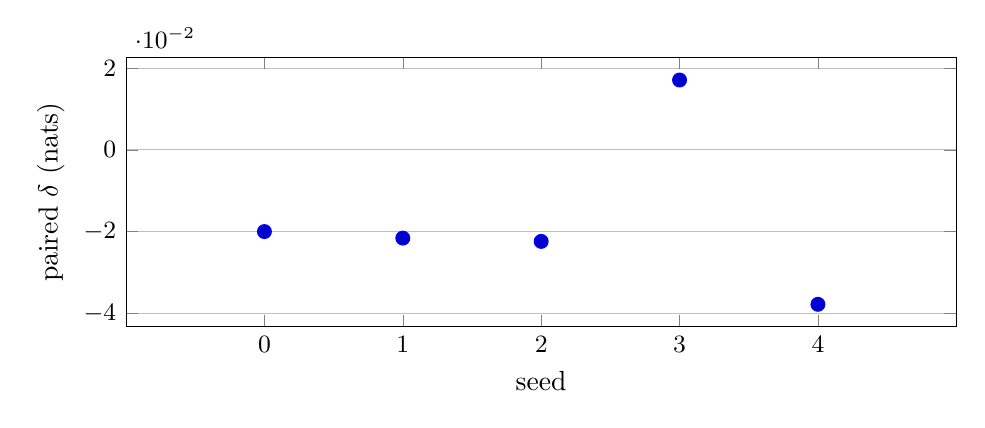
\begin{tikzpicture}
\begin{axis}[
  width=\linewidth, height=5cm, ylabel={paired $\delta$ (nats)},
  xlabel={seed}, xtick={0,1,2,3,4}, only marks,
  ymajorgrids, tick label style={font=\small},
]
\addplot+[mark=*, mark size=2.5pt] coordinates {(0,-0.0200) (1,-0.0216) (2,-0.0224) (3,0.0171) (4,-0.0378) };
\addplot[domain=-0.5:4.5, samples=2, dashed] {0};
\end{axis}
\end{tikzpicture}

\caption{The paired delta by seed. Negative favors differential
attention. The recorded single-seed win (seed 0) sits inside the band
of the four reruns, which includes a sign flip. Generated from the same
evidence as Table~\ref{tab:stage0}.}
\label{fig:band}
\end{figure}

\subsection{Stage 1: train-loss win, held-out loss}
At 162M parameters and 2.0B tokens the two loss signals disagree, and
the disagreement is the finding. Differential attention finishes
\StageOneTrainDeltaSigned{} nats ahead on train loss and
\StageOneValDeltaSigned{} nats behind on held-out validation
(Table~\ref{tab:stage1}, Figure~\ref{fig:curves}). The late run gives
it away. Over the final 5000 steps diff's val loss rises from
\StageOneDiffValLateRise{} nats while vanilla's falls from
\StageOneVanillaValLateFall{}. Diff is memorizing the training stream
harder, not learning a better function.

\begin{table}[tbp]
\centering
% GENERATED by gen.py. Do not edit.
\begin{tabular}{lrrr}
\toprule
metric & diff & vanilla & $\delta$ \\
\midrule
final train loss (last 1000-step mean) & 3.041 & 3.153 & -0.111 \\
held-out val loss at step 30000 & 3.362 & 3.326 & +0.035 \\
\bottomrule
\end{tabular}

\caption{Stage 1 (162M params, 2.0B tokens) endpoints, seed 0, paired
init, identical data order. Positive $\delta$ favors vanilla. Generated
from the released training logs.}
\label{tab:stage1}
\end{table}

\begin{figure}[tbp]
\centering
% GENERATED by gen.py. Do not edit.
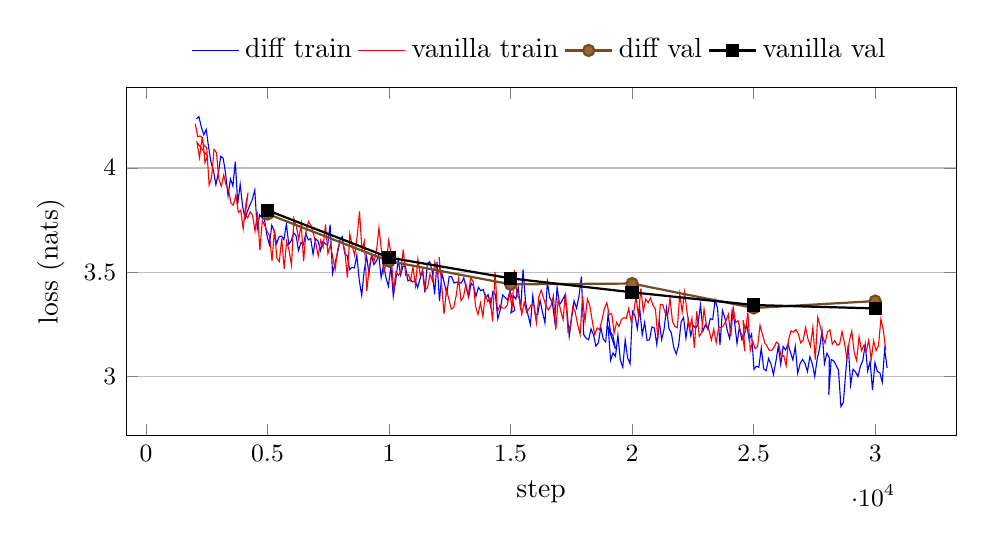
\begin{tikzpicture}
\begin{axis}[
  width=\linewidth, height=6cm, xlabel={step}, ylabel={loss (nats)},
  legend style={at={(0.5,1.04)},anchor=south,legend columns=-1,draw=none},
  ymajorgrids, tick label style={font=\small},
]
\addplot+[no marks, thin] coordinates {(2074,4.2348) (2174,4.2460) (2274,4.1971) (2374,4.1585) (2474,4.1852) (2574,4.1006) (2674,4.0265) (2774,3.9873) (2874,3.9195) (2974,3.9743) (3074,4.0555) (3174,4.0468) (3274,3.9729) (3374,3.8668) (3474,3.9475) (3574,3.9129) (3674,4.0303) (3774,3.8284) (3874,3.9219) (3974,3.8149) (4074,3.7552) (4174,3.7924) (4274,3.8222) (4374,3.8489) (4474,3.8937) (4574,3.7086) (4674,3.7750) (4774,3.7606) (4874,3.7519) (4974,3.6767) (5074,3.6329) (5174,3.7249) (5274,3.6972) (5374,3.6364) (5474,3.6710) (5574,3.6733) (5674,3.6568) (5774,3.7303) (5874,3.6338) (5974,3.6514) (6074,3.6895) (6174,3.6752) (6274,3.6038) (6374,3.6429) (6474,3.6315) (6574,3.6870) (6674,3.6549) (6774,3.6612) (6874,3.5869) (6974,3.6603) (7074,3.6503) (7174,3.6039) (7274,3.6470) (7374,3.6359) (7474,3.6308) (7574,3.7277) (7674,3.4933) (7774,3.5421) (7874,3.5877) (7974,3.6530) (8074,3.6705) (8174,3.5895) (8274,3.5800) (8374,3.5131) (8474,3.5234) (8574,3.5207) (8674,3.5818) (8774,3.4608) (8874,3.3887) (8974,3.5064) (9074,3.5752) (9174,3.4940) (9274,3.5801) (9374,3.5368) (9474,3.5527) (9574,3.5813) (9674,3.4741) (9774,3.5356) (9874,3.4733) (9974,3.4328) (10074,3.5302) (10174,3.3848) (10274,3.4605) (10374,3.5607) (10474,3.4865) (10574,3.5303) (10674,3.5276) (10774,3.4590) (10874,3.4634) (10974,3.4535) (11074,3.4606) (11174,3.4263) (11274,3.4682) (11374,3.5084) (11474,3.4029) (11574,3.5419) (11674,3.5500) (11774,3.5049) (11874,3.3942) (11974,3.5501) (12074,3.3621) (12174,3.4943) (12274,3.4476) (12374,3.3969) (12474,3.4794) (12574,3.4783) (12674,3.4481) (12774,3.4529) (12874,3.4505) (12974,3.4482) (13074,3.4728) (13174,3.4245) (13274,3.3795) (13374,3.4467) (13474,3.4347) (13574,3.3842) (13674,3.4275) (13774,3.4112) (13874,3.4176) (13974,3.3775) (14074,3.3927) (14174,3.3388) (14274,3.4073) (14374,3.3925) (14474,3.2768) (14574,3.3191) (14674,3.3913) (14774,3.3786) (14874,3.3668) (14974,3.4108) (15074,3.3720) (15174,3.3172) (15013,3.3057) (15113,3.3872) (15213,3.3715) (15313,3.4287) (15413,3.3191) (15513,3.5139) (15613,3.3598) (15713,3.2970) (15813,3.2490) (15913,3.3871) (16013,3.2995) (16113,3.2962) (16213,3.3657) (16313,3.3076) (16413,3.2573) (16513,3.4529) (16613,3.3765) (16713,3.3568) (16813,3.2689) (16913,3.4280) (17013,3.3445) (17113,3.3617) (17213,3.3863) (17313,3.3240) (17413,3.1925) (17513,3.2829) (17613,3.3628) (17713,3.3277) (17813,3.3843) (17913,3.4793) (18011,3.2003) (18111,3.1832) (18211,3.1762) (18311,3.2287) (18411,3.1996) (18511,3.1459) (18611,3.1618) (18711,3.2357) (18811,3.1800) (18911,3.1656) (19011,3.2981) (19111,3.2138) (19211,3.1961) (19311,3.1335) (19015,3.2360) (19115,3.0774) (19215,3.1128) (19315,3.0967) (19415,3.1977) (19515,3.0786) (19615,3.0445) (19715,3.1752) (19815,3.0892) (19915,3.0610) (20015,3.3123) (20115,3.2930) (20215,3.2297) (20315,3.3244) (20415,3.1993) (20515,3.2600) (20615,3.1727) (20715,3.1760) (20815,3.2376) (20915,3.2326) (21015,3.1534) (21115,3.2680) (21215,3.1769) (21315,3.2269) (21415,3.3280) (21515,3.2302) (21615,3.2083) (21715,3.1394) (21815,3.1078) (21915,3.1509) (22015,3.2606) (22115,3.2830) (22215,3.1842) (22315,3.2702) (22415,3.1946) (22515,3.2461) (22615,3.2317) (22715,3.2543) (22815,3.3443) (22915,3.2172) (23015,3.2483) (23115,3.2262) (23215,3.2773) (23315,3.2730) (23415,3.3671) (23515,3.3260) (23615,3.1522) (23715,3.3169) (23815,3.2820) (23915,3.2213) (24015,3.1812) (24115,3.3161) (24215,3.2612) (24315,3.1581) (24415,3.2377) (24515,3.1764) (24615,3.2004) (24715,3.2515) (24815,3.1756) (24915,3.2037) (25014,3.0346) (25114,3.0492) (25214,3.0449) (25314,3.1368) (25414,3.0362) (25514,3.0278) (25614,3.0864) (25714,3.0596) (25814,3.0097) (25914,3.0711) (26014,3.1459) (26114,3.0581) (26214,3.1437) (26314,3.1271) (26414,3.1567) (26514,3.1164) (26614,3.0797) (26714,3.1441) (26814,3.0155) (26914,3.0624) (27014,3.0821) (27114,3.0623) (27214,3.0237) (27314,3.0947) (27414,3.0613) (27514,3.0002) (27614,3.0837) (27714,3.1353) (27814,3.2202) (27914,3.0620) (28014,3.1116) (28114,3.0883) (28091,2.9130) (28191,3.0813) (28291,3.0753) (28391,3.0544) (28491,3.0304) (28591,2.8559) (28691,2.8751) (28791,3.0227) (28891,3.1521) (28991,2.9592) (29091,3.0349) (29191,3.0216) (29291,2.9997) (29391,3.0493) (29491,3.0767) (29591,3.1541) (29691,3.0262) (29791,3.0725) (29891,2.9350) (29991,3.0670) (30091,3.0237) (30191,3.0187) (30291,2.9730) (30391,3.1297) (30491,3.0414)};
\addplot+[no marks, thin] coordinates {(2025,4.2118) (2125,4.1501) (2225,4.1533) (2325,4.1454) (2425,4.0253) (2525,4.0569) (2097,4.1226) (2197,4.0496) (2297,4.1349) (2397,4.1067) (2497,4.0971) (2597,3.9181) (2697,3.9545) (2797,4.0887) (2897,4.0746) (2997,3.9458) (3097,3.9125) (3197,3.9660) (3297,3.9162) (3397,3.8925) (3497,3.8305) (3597,3.8222) (3697,3.8706) (3797,3.7868) (3897,3.7970) (3997,3.7088) (4097,3.8204) (4197,3.8812) (4084,3.7750) (4184,3.7606) (4284,3.7900) (4384,3.7722) (4484,3.6973) (4584,3.7902) (4684,3.6058) (4784,3.7485) (4884,3.7252) (4984,3.6950) (5084,3.6729) (5184,3.5549) (5284,3.7039) (5384,3.5662) (5484,3.5507) (5584,3.6620) (5684,3.5154) (5784,3.6476) (5884,3.6060) (5984,3.5346) (6084,3.7571) (6184,3.7211) (6284,3.6555) (6384,3.7328) (6484,3.5521) (6584,3.6969) (6684,3.7435) (6784,3.7246) (6884,3.6866) (6984,3.6372) (7084,3.5783) (7184,3.6534) (7284,3.6197) (7384,3.7290) (7484,3.5898) (7584,3.6300) (7684,3.5707) (7784,3.5149) (7884,3.6096) (7984,3.6447) (8084,3.6450) (8184,3.5996) (8284,3.4739) (8384,3.6839) (8484,3.6270) (8584,3.5799) (8684,3.6694) (8784,3.7912) (8884,3.6082) (8984,3.6484) (9084,3.4113) (9184,3.5234) (9284,3.5844) (9384,3.5549) (9484,3.6041) (9584,3.7138) (9684,3.6039) (9784,3.4985) (9884,3.5424) (9984,3.6527) (10084,3.5870) (10184,3.4108) (10284,3.5005) (10384,3.4851) (10484,3.4999) (10584,3.6098) (10684,3.4850) (10784,3.4900) (10884,3.4613) (10984,3.5240) (11084,3.4370) (11184,3.5620) (11284,3.4844) (11384,3.5115) (11484,3.4150) (11584,3.4270) (11684,3.4911) (11784,3.4595) (11884,3.5481) (11984,3.4896) (12084,3.5069) (12060,3.5735) (12160,3.4466) (12260,3.2997) (12360,3.4166) (12460,3.3717) (12560,3.3235) (12660,3.3308) (12760,3.3875) (12860,3.4700) (12960,3.3641) (13060,3.3807) (13160,3.4437) (13260,3.3907) (13360,3.4743) (13460,3.4553) (13560,3.3351) (13660,3.2976) (13760,3.3524) (13860,3.2870) (13960,3.3944) (14060,3.3591) (14160,3.3751) (14260,3.2629) (14360,3.5014) (14460,3.3104) (14560,3.3420) (14660,3.3282) (14760,3.3282) (14860,3.3408) (14960,3.4026) (15060,3.3287) (15160,3.5102) (15260,3.3931) (15360,3.3733) (15460,3.2980) (15560,3.3555) (15660,3.3090) (15760,3.3253) (15860,3.3458) (15960,3.3408) (16060,3.2576) (16160,3.3830) (16260,3.4133) (16360,3.3758) (16460,3.3373) (16560,3.3198) (16660,3.3390) (16760,3.3869) (16860,3.2248) (16960,3.3705) (17060,3.3161) (17160,3.2723) (17260,3.4026) (17360,3.2179) (17460,3.2452) (17560,3.3351) (17660,3.3085) (17760,3.2473) (17860,3.2012) (17960,3.3860) (18060,3.2634) (18160,3.3724) (18260,3.3391) (18360,3.2666) (18460,3.2009) (18560,3.2332) (18660,3.2233) (18760,3.2715) (18860,3.3271) (18960,3.3538) (19060,3.2960) (19160,3.3014) (19260,3.2086) (19360,3.2597) (19460,3.2400) (19560,3.2741) (19660,3.2819) (19760,3.2787) (19860,3.3256) (19960,3.2653) (20060,3.3022) (20160,3.3836) (20260,3.2909) (20360,3.4223) (20460,3.3126) (20560,3.3707) (20660,3.3537) (20760,3.3764) (20860,3.3399) (20960,3.3231) (21060,3.1782) (21160,3.3461) (21260,3.3446) (21360,3.3050) (21460,3.2884) (21560,3.3752) (21660,3.2638) (21760,3.2402) (21860,3.2339) (21960,3.3959) (22060,3.3091) (22160,3.4049) (22260,3.3102) (22360,3.2251) (22460,3.2790) (22560,3.1376) (22660,3.3127) (22760,3.1927) (22860,3.2094) (22960,3.3231) (23060,3.2449) (23160,3.2226) (23260,3.1747) (23360,3.2275) (23460,3.1622) (23560,3.2365) (23660,3.2337) (23760,3.2435) (23860,3.2672) (23960,3.2982) (24060,3.1926) (24160,3.3309) (24260,3.2592) (24360,3.2675) (24460,3.2116) (24538,3.1991) (24638,3.1213) (24563,3.2715) (24663,3.2216) (24763,3.3070) (24863,3.1239) (24963,3.1692) (25063,3.1327) (25163,3.1441) (25263,3.2450) (25363,3.2022) (25463,3.1600) (25537,3.1486) (25637,3.1264) (25737,3.1252) (25837,3.1393) (25937,3.1656) (26037,3.1534) (26137,3.0938) (26237,3.1006) (26337,3.0514) (26437,3.1775) (26537,3.2193) (26637,3.2131) (26737,3.2254) (26837,3.2056) (26937,3.1610) (27037,3.1737) (27137,3.2354) (27237,3.1799) (27337,3.1456) (27437,3.2357) (27537,3.0806) (27637,3.2832) (27737,3.2427) (27837,3.1933) (27937,3.1598) (28037,3.2137) (28137,3.2234) (28237,3.1552) (28337,3.1726) (28437,3.1503) (28537,3.1550) (28637,3.2159) (28737,3.1610) (28837,3.0855) (28937,3.1693) (29037,3.2180) (29137,3.1157) (29237,3.0764) (29337,3.1915) (29437,3.1235) (29537,3.1495) (29637,3.1225) (29737,3.1750) (29837,3.0815) (29937,3.1702) (30037,3.1236) (30137,3.1484) (30237,3.2766) (30337,3.2221) (30437,3.1259)};
\addplot+[mark=*, thick] coordinates {(5000,3.7794) (10000,3.5531) (15000,3.4420) (20000,3.4457) (25000,3.3285) (30000,3.3616)};
\addplot+[mark=square*, thick] coordinates {(5000,3.7968) (10000,3.5703) (15000,3.4706) (20000,3.4037) (25000,3.3427) (30000,3.3265)};
\legend{diff train, vanilla train, diff val, vanilla val}
\end{axis}
\end{tikzpicture}

\caption{Stage 1 train curves (thin, downsampled, from step 2000) and
held-out val points (marked). Diff holds the lower train loss
throughout while vanilla takes the lower val loss from mid-run on.
Generated from the released training logs.}
\label{fig:curves}
\end{figure}

\subsection{No positional structure in the delta}
Differential attention's pitch is that cancelling common-mode attention
noise matters most for long or noisy context, so its advantage should
grow with token position. We bin held-out negative log-likelihood by
position across the 2048-token window on both final checkpoints
(Table~\ref{tab:posbin}, Figure~\ref{fig:posbin}). Vanilla is ahead in
every bin. The delta is flat, spanning \PosbinMinDelta{} to
\PosbinMaxDelta{} nats with \PosbinLastBinDelta{} in the last bin, and
the overall gap of \PosbinOverallDelta{} nats matches the training-time
val gap measured on a different token budget. No widening with
position, no crossover at long range. The mechanism's designed
advantage does not appear in this regime.

\begin{table}[tbp]
\centering
% GENERATED by gen.py. Do not edit.
\begin{tabular}{lrrr}
\toprule
position & diff & vanilla & $\delta$ \\
\midrule
0--255 & 3.574 & 3.529 & +0.045 \\
256--511 & 3.380 & 3.341 & +0.039 \\
512--767 & 3.339 & 3.304 & +0.035 \\
768--1023 & 3.335 & 3.296 & +0.039 \\
1024--1279 & 3.323 & 3.287 & +0.036 \\
1280--1535 & 3.324 & 3.288 & +0.035 \\
1536--1791 & 3.333 & 3.297 & +0.035 \\
1792--2047 & 3.337 & 3.301 & +0.036 \\
\midrule
overall & 3.368 & 3.330 & +0.038 \\
\bottomrule
\end{tabular}

\caption{Held-out NLL by token position, both Stage 1 final
checkpoints. Positive $\delta$ favors vanilla. Generated from the
committed per-position evaluation.}
\label{tab:posbin}
\end{table}

\begin{figure}[tbp]
\centering
% GENERATED by gen.py. Do not edit.
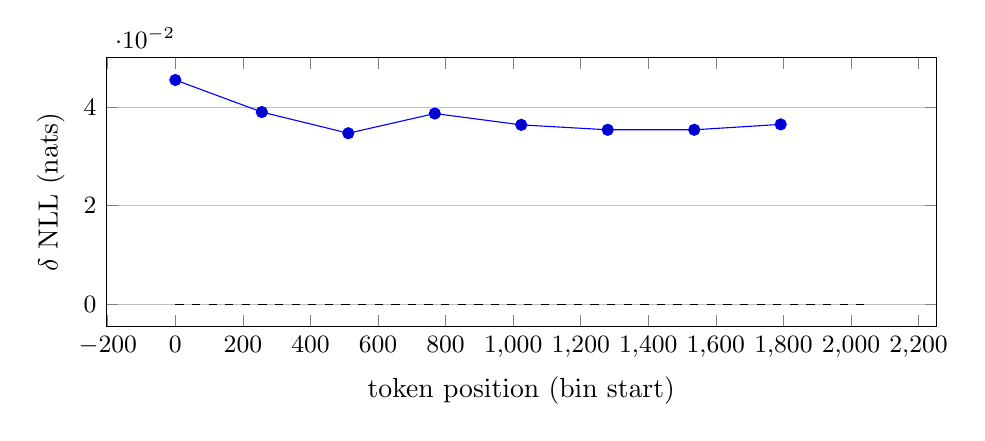
\begin{tikzpicture}
\begin{axis}[
  width=\linewidth, height=5cm, ylabel={$\delta$ NLL (nats)},
  xlabel={token position (bin start)},
  ymajorgrids, tick label style={font=\small},
]
\addplot+[mark=*] coordinates {(0,0.0455) (256,0.0390) (512,0.0347) (768,0.0387) (1024,0.0364) (1280,0.0354) (1536,0.0354) (1792,0.0365) };
\addplot[domain=0:2048, samples=2, dashed] {0};
\end{axis}
\end{tikzpicture}

\caption{The positional delta is flat. If common-mode cancellation
helped long context here, the curve would fall with position. Generated
from the same evidence as Table~\ref{tab:posbin}.}
\label{fig:posbin}
\end{figure}

\FloatBarrier

\section{Limitations}
Scale. This study sits three orders of magnitude below the original
paper's 3B-parameter, 1T-token setting. Nothing here refutes the
paper's results in its own regime. The claim is only that the benefit
is absent in ours.

Context and evals. The window is 2048 tokens and the metric is language
model loss. The paper's strongest results are long-context and
retrieval evals we do not run. The position-binned analysis is a proxy
for the long-context claim, not a replacement.

Seeds. The seed band is measured at Stage 0, where a run costs an hour.
Stage 1 remains a single seed. Its noise floor should be lower with
twenty times the tokens, and the overfitting signature is a mechanism
rather than a point estimate, but the Stage 1 delta does not carry a
measured band.

Data build. The four band seeds ran on a rebuilt tokenization with a
smaller held-out split than the original build. The band is internally
consistent. The recorded seed 0 delta crosses builds and carries that
caveat.

One machine, author-run. Training, evaluation, and analysis are all
ours, on hardware whose thermal and power behavior varied across runs
(Appendix~\ref{app:silicon}). Loss comparisons are unaffected. Wall
clock and throughput numbers are descriptive, not controlled.

\section{Conclusion}
At laptop scale, differential attention gave us nothing. A paired
seed band shows our initial small-scale win was seed noise, the
scaled-up run trades generalization for memorization, and the
positional profile shows no trace of the long-context advantage the
mechanism is designed for. The negative is bounded and honest. The
mechanism's reported gains live at a scale this study does not reach,
and anyone evaluating it below that scale should expect what we
measured, a delta indistinguishable from noise. The methodological
contribution stands apart from the negative. Byte-identical paired
initialization, a reference cross-check strict enough to catch
convention bugs, and a cross-stack replication make single-machine
architecture comparisons meaningful. Without them, our seed 0 result
would have been reported as a win.

\section{Availability}
Code (MIT), Metal kernels, the PyTorch cross-stack reference, training
logs, evaluation scripts, and both Stage 1 checkpoints are at
\url{https://github.com/guygrigsby/diff-mlx} and
\url{https://huggingface.co/guygrigsby/diff-mlx}.

\appendix
\section{Training on Apple Silicon}
\label{app:silicon}
Numbers a reader planning similar work will want. Sustained bf16
training of the 162M model on an M5 Max runs about 14k tokens per
second at context 2048, roughly 5 to 10 percent of nominal bf16 peak.
The workload is dispatch-bound, not compute-bound, which is what the
custom kernels target.

Per-token cost is flat in micro-batch until unified memory runs out,
then falls off a cliff. A micro-batch of 32 at Stage 1 exceeded the
128 GB ceiling and swap-thrashed to 950 tokens per second. Micro-batch
8 with gradient accumulation restored 14k. When a run is slow, check
swap before checking math.

Two throttles do not announce themselves. Under the stock fan curve a
closed laptop thermal-throttles within ten minutes of sustained
training. Forced fans and cross-flow hold throughput flat for days.
Separately, charging through a 100 W Thunderbolt dock instead of the
140 W first-party brick capped GPU clocks while the chip sat cool at
73$^\circ$C, with the battery slowly draining under a reported
charging state. A low temperature does not rule out throttling.
Confirm the negotiated adapter wattage before benchmarking, and state
cooling and power conditions with any published throughput number.

\bibliographystyle{plain}
\bibliography{references}

\end{document}
